% Exact LaTeX recreation of the supplied Phase-1.pdf
% Compile with pdfLaTeX. Place member pictures in the same folder if required.

\documentclass[11pt,a4paper]{article}

\usepackage[a4paper,left=2.0cm,right=2.0cm,top=1.55cm,bottom=1.55cm]{geometry}
\usepackage[T1]{fontenc}
\usepackage{lmodern}
\usepackage{graphicx}
\usepackage{xcolor}
\usepackage{array}
\usepackage{tabularx}
\usepackage{ragged2e}
\usepackage{enumitem}
\usepackage{fancyhdr}
\usepackage{tikz}
\usepackage{caption}
\usepackage{setspace}
\usepackage{url}

% -------------------------------------------------
% COLOURS
% -------------------------------------------------
\definecolor{TitleBlue}{RGB}{61,103,154}

% -------------------------------------------------
% GENERAL SETTINGS
% -------------------------------------------------
\setlength{\parindent}{0pt}
\setlength{\parskip}{0pt}
\renewcommand{\arraystretch}{1.0}

% The supplied document uses a clean sans-serif heading style
% and italic serif-style explanatory text.
\newcommand{\blueheading}[1]{%
    {\sffamily\color{TitleBlue}\fontsize{15}{18}\selectfont #1}%
}

\newcommand{\bluebigheading}[1]{%
    {\sffamily\bfseries\color{TitleBlue}\fontsize{16}{19}\selectfont #1}%
}

\newcommand{\instruction}[1]{%
    {\itshape\fontsize{10.5}{12.5}\selectfont #1}%
}

\newcommand{\answerbox}[2][3.0cm]{%
    \vspace{2pt}
    \noindent
    \fbox{%
        \begin{minipage}[t][#1][t]{\dimexpr\textwidth-2\fboxsep-2\fboxrule\relax}
            \vspace{1mm}
            \itshape #2
        \end{minipage}
    }
}

% -------------------------------------------------
% HEADER / FOOTER
% -------------------------------------------------
\pagestyle{fancy}
\fancyhf{}
\renewcommand{\headrulewidth}{0pt}
\renewcommand{\footrulewidth}{0pt}

\fancyhead[L]{%
    \sffamily\bfseries\itshape\fontsize{10.5}{12}\selectfont
    B. TECH CSE | DSCPP-III-2026-T376
}
\fancyhead[R]{%
    \sffamily\bfseries\fontsize{10.5}{12}\selectfont
    PROJECT PROPOSAL
}
\fancyfoot[R]{%
    \itshape\fontsize{10}{12}\selectfont
    Page \thepage
}
\setlength{\headheight}{14pt}
\setlength{\headsep}{23pt}
\setlength{\footskip}{24pt}

% -------------------------------------------------
% PAGE 1
% -------------------------------------------------
\begin{document}

\vspace{8mm}
\bluebigheading{PROJECT AND TEAM INFORMATION}

\vspace{13mm}

\blueheading{Project Title}

\vspace{1mm}

\answerbox[0.8cm]{\begin{center}
{\fontsize{14}{19}\selectfont\textbf{NetMind - Intelligent Network Traffic Analysis and Routing Engine}}
\end{center}}

\vspace{13mm}

\blueheading{Student / Team Information}

\vspace{2mm}

% Team information table
% Compact 4-member layout so all members remain on Page 1.
\noindent
\begin{tabularx}{\textwidth}{|>{\RaggedRight\arraybackslash}p{0.69\textwidth}|>{\RaggedRight\arraybackslash}X|}
\hline
\begin{minipage}[t]{\linewidth}
\vspace{1.5mm}
\textit{Team Name:}\\[-1mm]
\textit{Team \#}
\vspace{1.5mm}
\end{minipage}
&
\begin{minipage}[t]{\linewidth}
\vspace{1.5mm}
\textit{CodeGraphers}
\\
\textit{DSCPP-III-2026-T376}
\vspace{1.5mm}
\end{minipage}
\\
\hline
\begin{minipage}[t][3.25cm][t]{\linewidth}
\vspace{1.5mm}
\textbf{Team member 1 (Team Lead)}\\[-1mm]
\textit{(Last Name, name: student ID: email, picture):}
\vspace{2.0cm}
\end{minipage}
&
\begin{minipage}[t][3.25cm][t]{\linewidth}
\vspace{1.5mm}
\textit{Garg, Shristy -- 2510280123}\\
\textit{2510280123@geu.ac.in}

\vspace{2mm}
\includegraphics[width=3.0cm,height=1.5cm,keepaspectratio]{member1.jpeg}
\end{minipage}
\\
\hline
\begin{minipage}[t][3.25cm][t]{\linewidth}
\vspace{1.5mm}
\textbf{Team member 2}\\[-1mm]
\textit{(Last Name, name: student ID: email, picture):}
\vspace{2.0cm}
\end{minipage}
&
\begin{minipage}[t][3.25cm][t]{\linewidth}
\vspace{1.5mm}
\textit{Ojha, Gungun -- 2510012505}\\
\textit{2510012505@geu.ac.in}

\vspace{2mm}
\includegraphics[width=3.0cm,height=1.5cm,keepaspectratio]{member2.jpeg}
\end{minipage}
\\
\hline
\begin{minipage}[t][3.25cm][t]{\linewidth}
\vspace{1.5mm}
\textbf{Team member 3}\\[-1mm]
\textit{(Last Name, name: student ID: email, picture):}
\vspace{2.0cm}
\end{minipage}
&
\begin{minipage}[t][3.25cm][t]{\linewidth}
\vspace{1.5mm}
\textit{Mittra, Shrijit -- 2510370385}\\
\textit{2510370385@geu.ac.in}

\vspace{2mm}
\includegraphics[width=3.0cm,height=1.5cm,keepaspectratio]{member3.jpeg}
\end{minipage}
\\
\hline

\end{tabularx}

\vspace{3mm}

\begin{minipage}[t][3.25cm][t]{\linewidth}
\vspace{1.5mm}
\textbf{Mentor: }
\textit{Dr. Vidit Kumar}
\\
\textbf{Email: }
\textit{viditkumar.cse@geu.ac.in}
\end{minipage}

\newpage

% -------------------------------------------------
% PAGE 2
% -------------------------------------------------

\bluebigheading{PROPOSAL DESCRIPTION (10 pts)}

\vspace{7mm}

\blueheading{Motivation (1 pt)}

\vspace{1mm}

\answerbox[3cm]{Modern computer network process immense volume of daily traffic, making real-time monitoring and smart routing essential for reliability. While traditional simulation tool excel at logging individual metrics like latency, throughput, or jitter onto visual dashboards,they rarely go beyond passive observation.It remain difficult to see how network topologies, shifting traffic loads, and real-time routing decisions interact within a unified sandbox. NetMind solve this problem by putting network modeling, live traffic simulation, graph routing, and intelligent analytic into single cohesive system.\\
}

\vspace{7mm}

\blueheading{State of the Art / Current solution (1 pt)}

\vspace{1mm}

\answerbox[3.2cm]{Most modern network management tasks rely on specialized tools such as Wireshark, SolarWinds and Cisco Packet Tracer, which often fragment network analysis and hide routing logic behind black-box systems. NetMind address this gap through transparent,unified sandbox that expose classical routing algorithms , combines network modeling,packet-flow simulation and standard performance metrics ,and apply ML with historical context to detect anomalies, forecast traffic change and explain network decisions,allowing users to test scenarios, compare performance and understand the mechanics of network behavior .
}

\vspace{7mm}

\blueheading{Project Goals and Milestones (2 pts)}

\vspace{1mm}

\answerbox[6cm]{ 
NetMind is a graph-based engine designed for model network entities—such as host, routers, link, and flows—as dynamic graphs that simulates live traffic, congestion, and link failure. By tracking core performance metrics and macro characteristic, the platform run head-to-head evaluation of routing algorithms while deploying ML models to detect anomaly, analyze traffic pattern, and forecast future network state , additionally integrating GraphRAG layer for contextual analysis of topologies and historical event logs .
\\
The project milestones involves mapping system architectures, setting up core classes, and coding primary network graph engine for handles topology mapping, traversals, and packet-flow traffic simulations. Furthermore, team will integrating performance metrics, implement pathfinding routing engines, and cleans simulation datas to train Python ML models for anomaly detections. Finally, the project construct GraphRAG knowledge base to enabling contextual query, develop frontend visualisation dashboard, and finalising system documentations for project demo .
}

\vspace{7mm}

\blueheading{Project Approach (3 pts)}

\vspace{1mm}

\answerbox[5cm]{NetMind will be develop as modular layered system integrating networking, OOP,data structures, simulation, ML,and graph knowledge retrieval. Built using C++, the network engine uses object-oriented classes like router, host, and link while representing topologys through adjacency lists, priority queues, and hash map. The traffic simulation engine process packet and flow events under changing conditions—such as latencys, congestions,and link failure—to collecting metrics at the link and host level for evaluating pathfinding algorithms under identical scenario. Furthermore, Python ML pipeline utilizing Pandas, NumPy, Scikit-learn trains on simulation datasets to detects anomaly and forecast future network state, while GraphRAG layer connect topology and historical logs to enable context-aware querying, ultimately presenting real-time traffic paths and analytical results on a visualisation dashboard.
}

\newpage

% -------------------------------------------------
% PAGE 3
% -------------------------------------------------

\blueheading{System Architecture (High Level Diagram)(2 pts)}

\vspace{3mm}

\begin{center}

\begin{tikzpicture}[
    box/.style={
        rectangle,
        draw=TitleBlue,
        thick,
        rounded corners=3pt,
        align=center,
        minimum width=38mm,
        minimum height=11mm,
        font=\itshape\fontsize{10.5}{12.5}\selectfont
    },
    arrow/.style={
        ->,
        thick
    },
    dashedarrow/.style={
        ->,
        thick,
        dashed
    }
]

\node[box] (user) at (-2.5,0)
    {User / Network Analyst};

\node[box] (interface) at (2.5,0)
    {Visualization \&\\Interactive Interface};


\node[box] (controller) at (0,-2)
    {Application Controller\\\& Scenario Manager};


\node[box] (network) at (-4,-4.2)
    {Network Model\\
     \scriptsize Routers, Hosts, Links, Packets};

\node[box] (graph) at (4,-4.2)
    {Graph \& DSA Engine\\
     \scriptsize BFS, DFS, Graph Structures};


\node[box] (routing) at (-4,-6.5)
    {Routing Engine\\
     \scriptsize Dijkstra \& Alternative Algorithms};

\node[box] (simulation) at (4,-6.5)
    {Traffic Simulation Engine\\
     \scriptsize Traffic, Queues, Congestion, Failures};


\node[box] (metrics) at (0,-8.8)
    {Network Metrics \& Analytics\\
     \scriptsize Throughput, Latency, Jitter, Loss, Utilization};


\node[box] (storage) at (0,-11.2)
    {Data \& Experiment Storage\\
     \scriptsize Metrics, Traffic, Events, Topology, History};


\node[box] (ml) at (-4,-14.2)
    {Machine Learning\\
     \scriptsize Traffic Patterns, Anomaly Detection, Prediction};

\node[box] (rag) at (4,-14.2)
    {GraphRAG / Knowledge Layer\\
     \scriptsize Knowledge Graph, Retrieval, Explanations};


\draw[arrow] (user) -- (interface);
\draw[arrow] (interface) -- (user);

\draw[arrow] (interface) -- (controller);
\draw[arrow] (controller) -- (interface);


\draw[arrow] (controller) -- (network);
\draw[arrow] (controller) -- (graph);


\draw[arrow] (network) -- (routing);
\draw[arrow] (graph) -- (routing);

\draw[arrow] (network) -- (simulation);
\draw[arrow] (routing) -- (simulation);
\draw[arrow] (graph) -- (simulation);


\draw[arrow] (routing) -- (metrics);
\draw[arrow] (simulation) -- (metrics);


\draw[arrow] (metrics) -- (storage);


\draw[arrow] (storage) -- (ml);
\draw[arrow] (storage) -- (rag);


\draw[arrow]
    (ml.west)
    -- (-8,-14.2)
    -- (-8,-2)
    -- (controller.west);

\draw[arrow]
    (rag.east)
    -- (8,-14.2)
    -- (8,-2)
    -- (controller.east);

\end{tikzpicture}

\end{center}

\begin{center}
\small
\textit{Figure: High-Level System Architecture of NetMind}
\end{center}

\vspace{300mm}

\blueheading{Project Outcome / Deliverables (1 pts)}

\vspace{1mm}

\answerbox[4.2cm] {
The main outcome of the NetMind project is a working prototype of an intelligent network traffic analysis, simulation, and routing system based on classical networking algorithms and data-driven analysis.
\\
The project will deliver a C++ OOP network modelling \& graph engine to represent network infrastructure, nodes and links,a traffic simulation for modelling congestion, delays,packet loss and link failures, a routing module for comparing different routing algorithm, a dashboard to visualise different network metrics, a ML pipeline for forecasting network conditions, a GraphRAG knowledge layer for context aware analysis using topology and historical log.

}

\vspace{7mm}

\blueheading{Assumptions}

\vspace{1mm}

\answerbox[4cm]{The project assumes a simulated network environment in which routers, hosts, links, and traffic flows can be modelled. Link characteristics such as bandwidth, latency, and packet loss may remain fixed or vary according to predefined scenarios. Routing algorithms will be evaluated under identical network conditions to ensure fair comparison, while ML models will be trained using data generated from simulations in similar environments. The GraphRAG layer will use the network data and knowledge graph generated during system evaluation to support contextual analysis. Overall, NetMind focuses on network simulation and analysis rather than configuration or optimisation of real-world network infrastructure.}

\vspace{7mm}

\blueheading{References}

\vspace{1mm}

\answerbox[6cm]{

> Harvard CS145 — Routing Network Simulator\newline
\url{https://github.com/Harvard-CS145/routing}

> NetSimCPP — C++ Network Simulator\newline
\url{https://github.com/UmarlyPoeta/inzynieria_oprogramowania}

> Wireshark — Network Protocol Analyzer and Packet Analysis Resources\newline
\url{https://www.wireshark.org/}

> Microsoft GraphRAG\newline
\url{https://github.com/microsoft/graphrag}

> Flow simulator -- C++\newline
\url{https://github.com/jianglong-nie/Flow-Simulator}

> From statistical- to machine learning-based network traffic prediction\newline
\url{https://onlinelibrary.wiley.com/doi/10.1002/ett.4394}

}
\end{document}
